%%%%%%%%%%%%%%%%%%%%%%%%%%%%%%%%%%%%%%%%%
%----------------------------------------------------------------------------------------
%	PACKAGES AND OTHER DOCUMENT CONFIGURATIONS
%----------------------------------------------------------------------------------------

\documentclass[12pt]{article}

\usepackage{amsmath}

\usepackage{graphicx}

\usepackage{hyperref}

\usepackage[utf8]{inputenc}

%%%%%%%%%%%%%%%%%%%%%%%%%%%%%%%%%%%%%%%%%
% Arsclassica Article
% Structure Specification File
%
% This file has been downloaded from:
% http://www.LaTeXTemplates.com
%
% Original author:
% Lorenzo Pantieri (http://www.lorenzopantieri.net) with extensive modifications by:
% Vel (vel@latextemplates.com)
%
% License:
% CC BY-NC-SA 3.0 (http://creativecommons.org/licenses/by-nc-sa/3.0/)
%
%%%%%%%%%%%%%%%%%%%%%%%%%%%%%%%%%%%%%%%%%

%----------------------------------------------------------------------------------------
%	REQUIRED PACKAGES
%----------------------------------------------------------------------------------------

\usepackage[
nochapters, % Turn off chapters since this is an article        
beramono, % Use the Bera Mono font for monospaced text (\texttt)
eulermath,% Use the Euler font for mathematics
pdfspacing, % Makes use of pdftex’ letter spacing capabilities via the microtype package
dottedtoc % Dotted lines leading to the page numbers in the table of contents
]{classicthesis} % The layout is based on the Classic Thesis style

\usepackage{arsclassica} % Modifies the Classic Thesis package

\usepackage[T1]{fontenc} % Use 8-bit encoding that has 256 glyphs

\usepackage[utf8]{inputenc} % Required for including letters with accents

\usepackage{graphicx} % Required for including images
\graphicspath{{Figures/}} % Set the default folder for images

\usepackage{enumitem} % Required for manipulating the whitespace between and within lists

\usepackage{lipsum} % Used for inserting dummy 'Lorem ipsum' text into the template

\usepackage{subfig} % Required for creating figures with multiple parts (subfigures)

\usepackage{amsmath,amssymb,amsthm} % For including math equations, theorems, symbols, etc

\usepackage{varioref} % More descriptive referencing

\usepackage{makeidx}
%----------------------------------------------------------------------------------------
%	THEOREM STYLES
%---------------------------------------------------------------------------------------

\theoremstyle{definition} % Define theorem styles here based on the definition style (used for definitions and examples)
\newtheorem{definition}{Definition}

\theoremstyle{plain} % Define theorem styles here based on the plain style (used for theorems, lemmas, propositions)
\newtheorem{theorem}{Theorem}

\theoremstyle{remark} % Define theorem styles here based on the remark style (used for remarks and notes)

%----------------------------------------------------------------------------------------
%	HYPERLINKS
%---------------------------------------------------------------------------------------

\hypersetup{
%draft, % Uncomment to remove all links (useful for printing in black and white)
colorlinks=true, breaklinks=true, bookmarks=true,bookmarksnumbered,
urlcolor=webbrown, linkcolor=RoyalBlue, citecolor=webgreen, % Link colors
pdftitle={Darkly: There is something wrong...}, % PDF title
pdfauthor={Sibonelo Nkosi \textcopyright}, % PDF Author
pdfsubject={Web Security}, % PDF Subject
pdfkeywords={WeThinkCode}, % PDF Keywords
pdfcreator={pdfLaTeX}, % PDF Creator
pdfproducer={LaTeX with hyperref and ClassicThesis} % PDF producer
} % Include the structure.tex file which specified the document structure and layout

\hyphenation{Fortran hy-phen-ation} % Specify custom hyphenation points in words with dashes where you would like hyphenation to occur, or alternatively, don't put any dashes in a word to stop hyphenation altogether
%----------------------------------------------------------------------------------------
%	CODE SNIPPET INSERTION
\usepackage{listings} % Required for inserting code snippets
%\usepackage[usenames,dvipsnames]{color} % Required for specifying custom colors and referring to colors by name

\definecolor{DarkGreen}{rgb}{0.0,0.4,0.0} % Comment color
\definecolor{highlight}{RGB}{255,251,204} % Code highlight color

\lstdefinestyle{Style1}{ % Define a style for your code snippet, multiple definitions can be made if, for example, you wish to insert multiple code snippets using different programming languages into one document
language=Perl, % Detects keywords, comments, strings, functions, etc for the language specified
backgroundcolor=\color{highlight}, % Set the background color for the snippet - useful for highlighting
basicstyle=\footnotesize\ttfamily, % The default font size and style of the code
breakatwhitespace=false, % If true, only allows line breaks at white space
breaklines=true, % Automatic line breaking (prevents code from protruding outside the box)
captionpos=b, % Sets the caption position: b for bottom; t for top
commentstyle=\usefont{T1}{pcr}{m}{sl}\color{DarkGreen}, % Style of comments within the code - dark green courier font
deletekeywords={}, % If you want to delete any keywords from the current language separate them by commas
%escapeinside={\%}, % This allows you to escape to LaTeX using the character in the bracket
firstnumber=1, % Line numbers begin at line 1
frame=single, % Frame around the code box, value can be: none, leftline, topline, bottomline, lines, single, shadowbox
frameround=tttt, % Rounds the corners of the frame for the top left, top right, bottom left and bottom right positions
keywordstyle=\color{Blue}\bf, % Functions are bold and blue
morekeywords={}, % Add any functions no included by default here separated by commas
numbers=left, % Location of line numbers, can take the values of: none, left, right
numbersep=10pt, % Distance of line numbers from the code box
numberstyle=\tiny\color{Gray}, % Style used for line numbers
rulecolor=\color{black}, % Frame border color
showstringspaces=false, % Don't put marks in string spaces
showtabs=false, % Display tabs in the code as lines
stepnumber=5, % The step distance between line numbers, i.e. how often will lines be numbered
stringstyle=\color{Purple}, % Strings are purple
tabsize=2, % Number of spaces per tab in the code
}

% Create a command to cleanly insert a snippet with the style above anywhere in the document
\newcommand{\insertcode}[2]{\begin{itemize}\item[]\lstinputlisting[caption=#2,label=#1,style=Style1]{#1}\end{itemize}} % The first argument is the script location/filename and the second is a caption for the listing
%----------------------------------------------------------------------------------------

\makeindex
\begin{document}

%----------------------------------------------------------------------------------------
%	HEADERS
%----------------------------------------------------------------------------------------

\renewcommand{\sectionmark}[1]{\markright{\spacedlowsmallcaps{#1}}} % The header for all pages (oneside) or for even pages (twoside)
%\renewcommand{\subsectionmark}[1]{\markright{\thesubsection~#1}} % Uncomment when using the twoside option - this modifies the header on odd pages
\lehead{\mbox{\llap{\small\thepage\kern1em\color{halfgray} \vline}\color{halfgray}\hspace{0.5em}\rightmark\hfil}} % The header style

\pagestyle{scrheadings} % Enable the headers specified in this block

%%%%%%%%%%%%%%%%%%%%%%%%%%%%%%%%%%%%%%%%%
% Academic Title Page
% LaTeX Template
% Version 2.0 (17/7/17)
%
% 
%
%%%%%%%%%%%%%%%%%%%%%%%%%%%%%%%%%%%%%%%%%

%----------------------------------------------------------------------------------------
%	PACKAGES AND OTHER DOCUMENT CONFIGURATIONS
%----------------------------------------------------------------------------------------

%\documentclass[11pt]{article}

%\usepackage[utf8]{inputenc} % Required for inputting international characters
%\usepackage[T1]{fontenc} % Output font encoding for international characters

%\usepackage{mathpazo} % Palatino font

%\begin{document}

%----------------------------------------------------------------------------------------
%	TITLE PAGE
%----------------------------------------------------------------------------------------

\begin{titlepage} % Suppresses displaying the page number on the title page and the subsequent page counts as page 1
	\newcommand{\HRule}{\rule{\linewidth}{0.5mm}} % Defines a new command for horizontal lines, change thickness here
	
	\center % Centre everything on the page
	
	%------------------------------------------------
	%	Headings
	%------------------------------------------------
	
	\textsc{\LARGE WeThinkCode\_}\\[1.5cm] % Main heading such as the name of your university/college
	
	\textsc{\Large WEB II}\\[0.5cm] % Major heading such as course name
	
	\textsc{\large Project II}\\[0.5cm] % Minor heading such as course title
	
	%------------------------------------------------
	%	Title
	%------------------------------------------------
	
	\HRule\\[0.4cm]
	
	{\huge\bfseries Darkly: }\\{\large There is something wrong...}\\[0.4cm] % Title of your document
	
	\HRule\\[1.5cm]
	
	%------------------------------------------------
	%	Author(s)
	%------------------------------------------------
	
	% \begin{minipage}{0.4\textwidth}
	% 	\begin{flushleft}
	% 		\large
	% 		\textit{Developer}\\
	% 		Mosima \textsc{Mamaleka} % Your name
	% 	\end{flushleft}
	% \end{minipage}
	% ~
	% \begin{minipage}{0.4\textwidth}
	% 	\begin{flushright}
	% 		\large
	% 		\textit{Developer}\\
	% 		Sibonelo \textsc{Nkosi} % Supervisor's name
	% 	\end{flushright}
	% \end{minipage}
	
	% If you don't want a supervisor, uncomment the two lines below and comment the code above
	{\large\textit{Developer}}\\
	Sibonelo \textsc{Nkosi}\\ % Your name
	Username: \textsc{sinkosi} % Your name

	\vfill
	{\large\textit{Assessor}}\\
	Mufaro \textsc{Simbisayi}\\ % Your name
	%------------------------------------------------
	%	Date
	%------------------------------------------------
	
	\vfill\vfill\vfill % Position the date 3/4 down the remaining page
	
	\large{October 2020}\\ % Date, change the \today to a set date if you want to be precise
	
	%------------------------------------------------
	%	Logo
	%------------------------------------------------
	
	\vfill\vfill
	
	
\includegraphics[width=0.2\textwidth]{0.title/index.png}\\[1cm] % Include a department/university logo - this will require the graphicx package
	
\includegraphics[width=0.2\textwidth]{0.title/docker.png}\\[1cm] % Include a department/university logo - this will require the graphicx package
	%----------------------------------------------------------------------------------------
	
	\vfill % Push the date up 1/4 of the remaining page
	
\end{titlepage}

%----------------------------------------------------------------------------------------

%\end{document}


%----------------------------------------------------------------------------------------
%	TABLE OF CONTENTS & LISTS OF FIGURES AND TABLES
%----------------------------------------------------------------------------------------
\newpage
%\maketitle % Print the title/author/date block

\setcounter{tocdepth}{3} % Set the depth of the table of contents to show sections and subsections only

\tableofcontents % Print the table of contents

\newpage

%\listoffigures % Print the list of figures

%\listoftables % Print the list of tables


%----------------------------------------------------------------------------------------
%	ABSTRACT
%----------------------------------------------------------------------------------------

\newpage

\section{Introduction}

The aim of this project is to introduce you to computer security in the web domain.
You will be able to discover OWASP, which is, no more and no less, the biggest web
security project to date.
You will also understand what a lot of frameworks do in an automatic and completely
transparent way for you.

You will need to use a virtual machine (i386) to validate this project. Once your
machine is started with the ISO supplied with the subject.
Requirements:
\begin{itemize}
    \item Virtual Box
    \item darkly.iso (\href{https://drive.google.com/file/d/145dbZHjZWyMiRscj-72jE3n5PM5vXyB9/view?usp=sharing}{download here} )
    \item Other stuff
\end{itemize}

\section{Getting Started}

\subsection{Windows}
Windows Installation\textsuperscript{*}: Windows is trash\cite{Docker:Windows_Install}

%----------------------------------------------------------------------------------------
%	Footnotes
%----------------------------------------------------------------------------------------

\let\thefootnote\relax\footnotetext{\textsuperscript{*} \textit{Information provided is correct for current users configuration i.e Windows Home 10:2004, results
may differ for other configurations }}
\let\thefootnote\relax\footnotetext{\textsuperscript{**} \textit{Snap install is not available for all Linux Distros, this is expected to work on Ubuntu and Debian flavours}}
%----------------------------------------------------------------------------------------
\subsection{Linux}
\noindent Linux Installation\textsuperscript{**}: Begin by ensuring that you have Virtual Box installed on your system, if not type:
\begin{lstlisting}[language=bash]
    $ sudo apt-get install virtualbox
\end{lstlisting}
%\vfill
\begin{figure}[!htb]
    \centering
    %\insertcode{Scripts/example.pl}{Nena would be proud.} % The first argument is the script location/filename and the second is a caption for the listing
    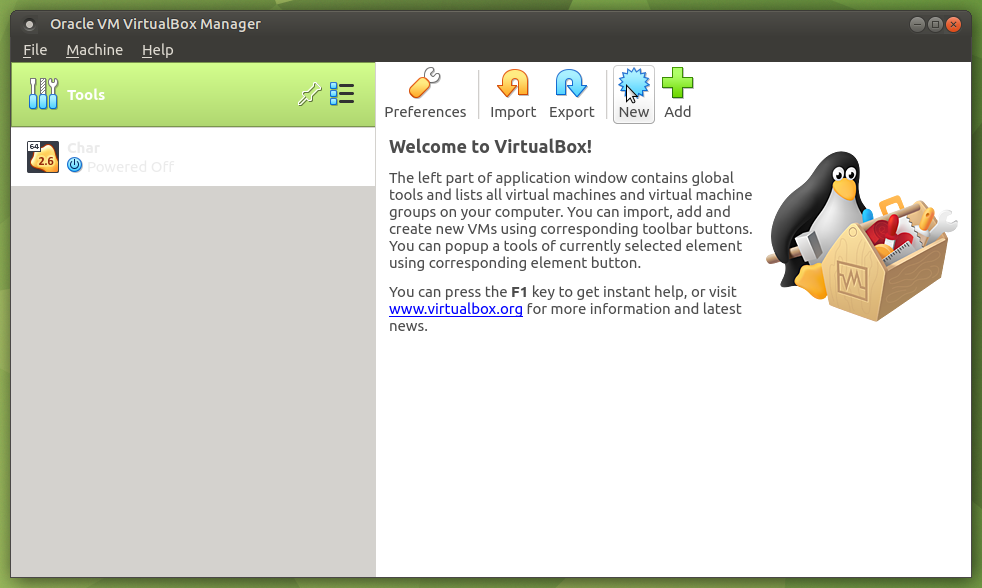
\includegraphics[width=0.752\textwidth]{images/00-0.png}\\[0cm]  
    \caption[Virtual Box]{\emph{Virtual Box Landing}, on Ubuntu}
    %from \url{http://localhost:3000/}).} % The text in the square bracket is the caption for the list of figures while the text in the curly brackets is the figure caption
    \label{fig:00-01 - Linux Virtual Box Landing} 
\end{figure}

\subsubsection{New Virtual Machine}

\begin{figure}[!htb]
    \centering
    %\insertcode{Scripts/example.pl}{Nena would be proud.} % The first argument is the script location/filename and the second is a caption for the listing
    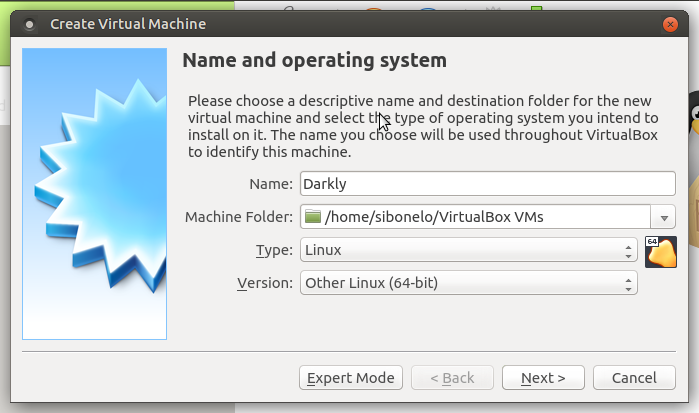
\includegraphics[width=0.752\textwidth]{images/00-01.png}\\[0cm]  
    \caption[Virtual Box]{\emph{Virtual Box Landing}, on Ubuntu}
    %from \url{http://localhost:3000/}).} % The text in the square bracket is the caption for the list of figures while the text in the curly brackets is the figure caption
    \label{fig:00-01 - Linux Virtual Box New VM} 
\end{figure}
Begin by installing a new

\subsubsection{Linux}

\begin{figure}[!htb]
    \centering
    %\insertcode{Scripts/example.pl}{Nena would be proud.} % The first argument is the script location/filename and the second is a caption for the listing
    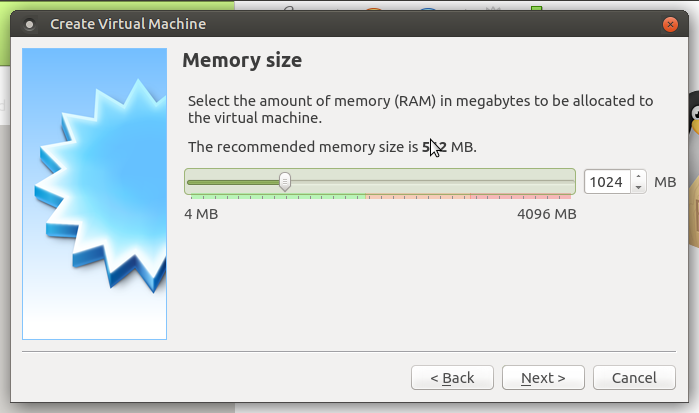
\includegraphics[width=0.752\textwidth]{images/00-02.png}\\[0cm]  
    \caption[Virtual Box]{\emph{Virtual Box Landing}, on Ubuntu}
    %from \url{http://localhost:3000/}).} % The text in the square bracket is the caption for the list of figures while the text in the curly brackets is the figure caption
    \label{fig:00-02 - Linux Virtual Box Landing} 
\end{figure}

Tell the system to use Linu
\subsubsection{Linux}

\begin{figure}[!htb]
    \centering
    %\insertcode{Scripts/example.pl}{Nena would be proud.} % The first argument is the script location/filename and the second is a caption for the listing
    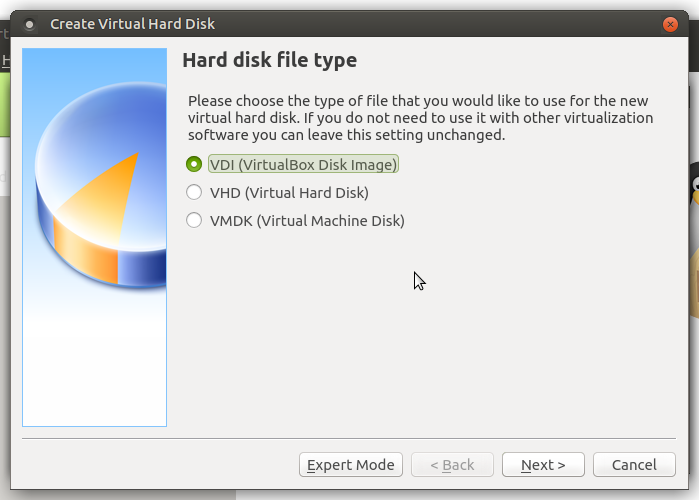
\includegraphics[width=0.752\textwidth]{images/00-03.png}\\[0cm]  
    \caption[Virtual Box]{\emph{Virtual Box Landing}, on Ubuntu}
    %from \url{http://localhost:3000/}).} % The text in the square bracket is the caption for the list of figures while the text in the curly brackets is the figure caption
    \label{fig:00-03 - Linux Virtual Box Landing} 
\end{figure}

Tell the system to use Linu
\subsubsection{Linux}

\begin{figure}[!htb]
    \centering
    %\insertcode{Scripts/example.pl}{Nena would be proud.} % The first argument is the script location/filename and the second is a caption for the listing
    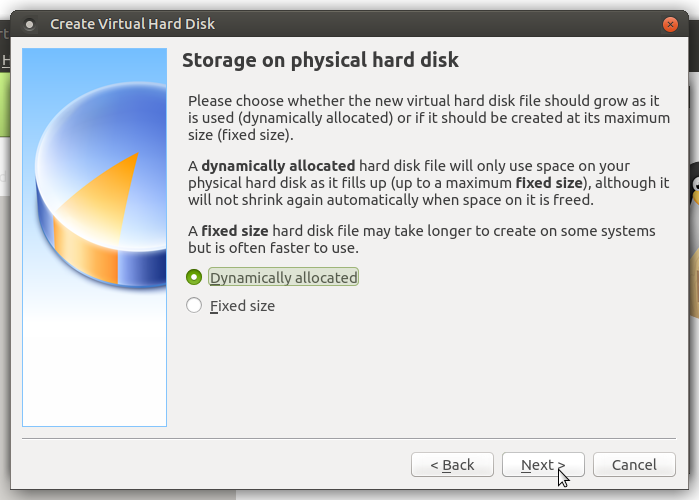
\includegraphics[width=0.752\textwidth]{images/00-04.png}\\[0cm]  
    \caption[Virtual Box]{\emph{Virtual Box Landing}, on Ubuntu}
    %from \url{http://localhost:3000/}).} % The text in the square bracket is the caption for the list of figures while the text in the curly brackets is the figure caption
    \label{fig:00-04 - Linux Virtual Box Landing} 
\end{figure}

Tell the system to use Linu
\subsubsection{Linux}

\begin{figure}[!htb]
    \centering
    %\insertcode{Scripts/example.pl}{Nena would be proud.} % The first argument is the script location/filename and the second is a caption for the listing
    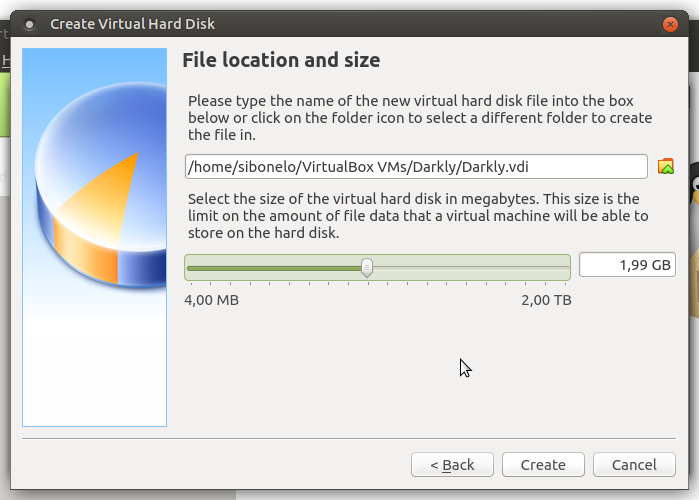
\includegraphics[width=0.752\textwidth]{images/00-05.png}\\[0cm]  
    \caption[Virtual Box]{\emph{Virtual Box Landing}, on Ubuntu}
    %from \url{http://localhost:3000/}).} % The text in the square bracket is the caption for the list of figures while the text in the curly brackets is the figure caption
    \label{fig:00-05 - Linux Virtual Box Landing} 
\end{figure}

Tell the system to use Linu
\subsubsection{Linux}

\begin{figure}[!htb]
    \centering
    %\insertcode{Scripts/example.pl}{Nena would be proud.} % The first argument is the script location/filename and the second is a caption for the listing
    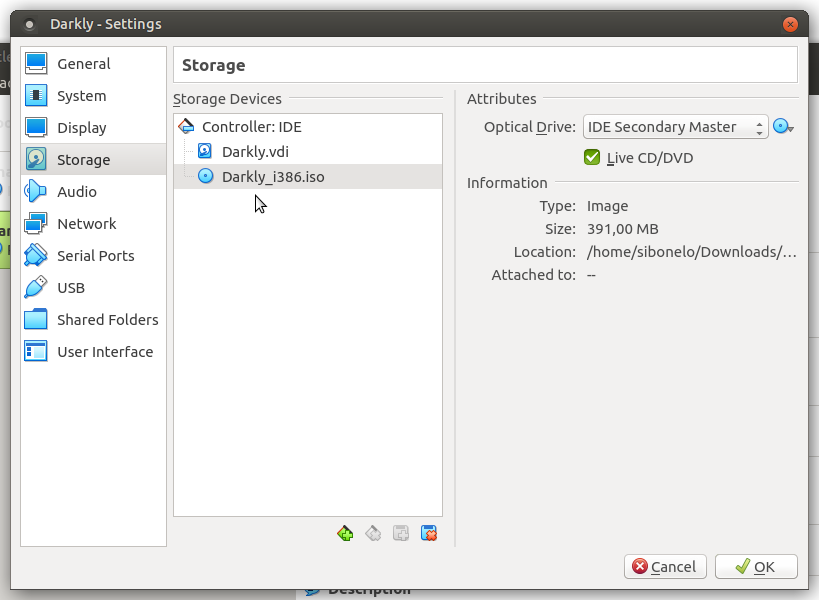
\includegraphics[width=0.752\textwidth]{images/00-06.png}\\[0cm]  
    \caption[Virtual Box]{\emph{Virtual Box Landing}, on Ubuntu}
    %from \url{http://localhost:3000/}).} % The text in the square bracket is the caption for the list of figures while the text in the curly brackets is the figure caption
    \label{fig:00-06 - Linux Virtual Box Landing} 
\end{figure}

Tell the system to use Linu
\subsubsection{Linux}

\begin{figure}[!htb]
    \centering
    %\insertcode{Scripts/example.pl}{Nena would be proud.} % The first argument is the script location/filename and the second is a caption for the listing
    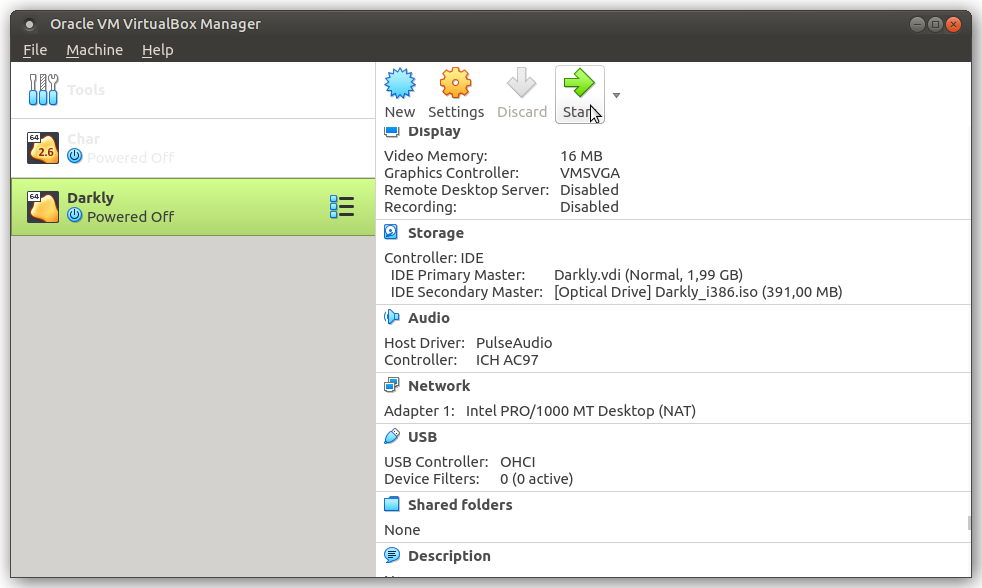
\includegraphics[width=0.752\textwidth]{images/00-07.png}\\[0cm]  
    \caption[Virtual Box]{\emph{Virtual Box Landing}, on Ubuntu}
    %from \url{http://localhost:3000/}).} % The text in the square bracket is the caption for the list of figures while the text in the curly brackets is the figure caption
    \label{fig:00-07 - Linux Virtual Box Landing} 
\end{figure}

Tell the system to use Linu
\subsubsection{Linux}

\begin{figure}[!htb]
    \centering
    %\insertcode{Scripts/example.pl}{Nena would be proud.} % The first argument is the script location/filename and the second is a caption for the listing
    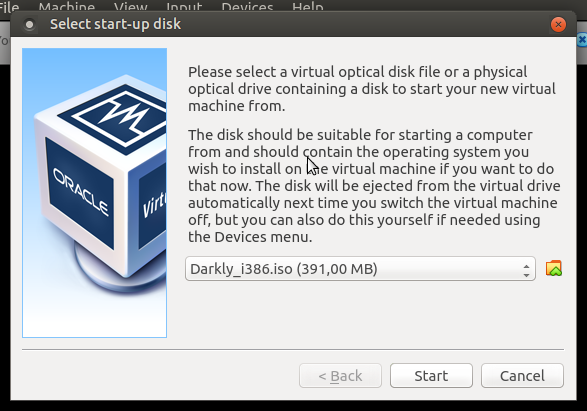
\includegraphics[width=0.752\textwidth]{images/00-08.png}\\[0cm]  
    \caption[Virtual Box]{\emph{Virtual Box Landing}, on Ubuntu}
    %from \url{http://localhost:3000/}).} % The text in the square bracket is the caption for the list of figures while the text in the curly brackets is the figure caption
    \label{fig:00-08 - Linux Virtual Box Landing} 
\end{figure}

Tell the system to use Linu
\subsubsection{Linux}

\begin{figure}[!htb]
    \centering
    %\insertcode{Scripts/example.pl}{Nena would be proud.} % The first argument is the script location/filename and the second is a caption for the listing
    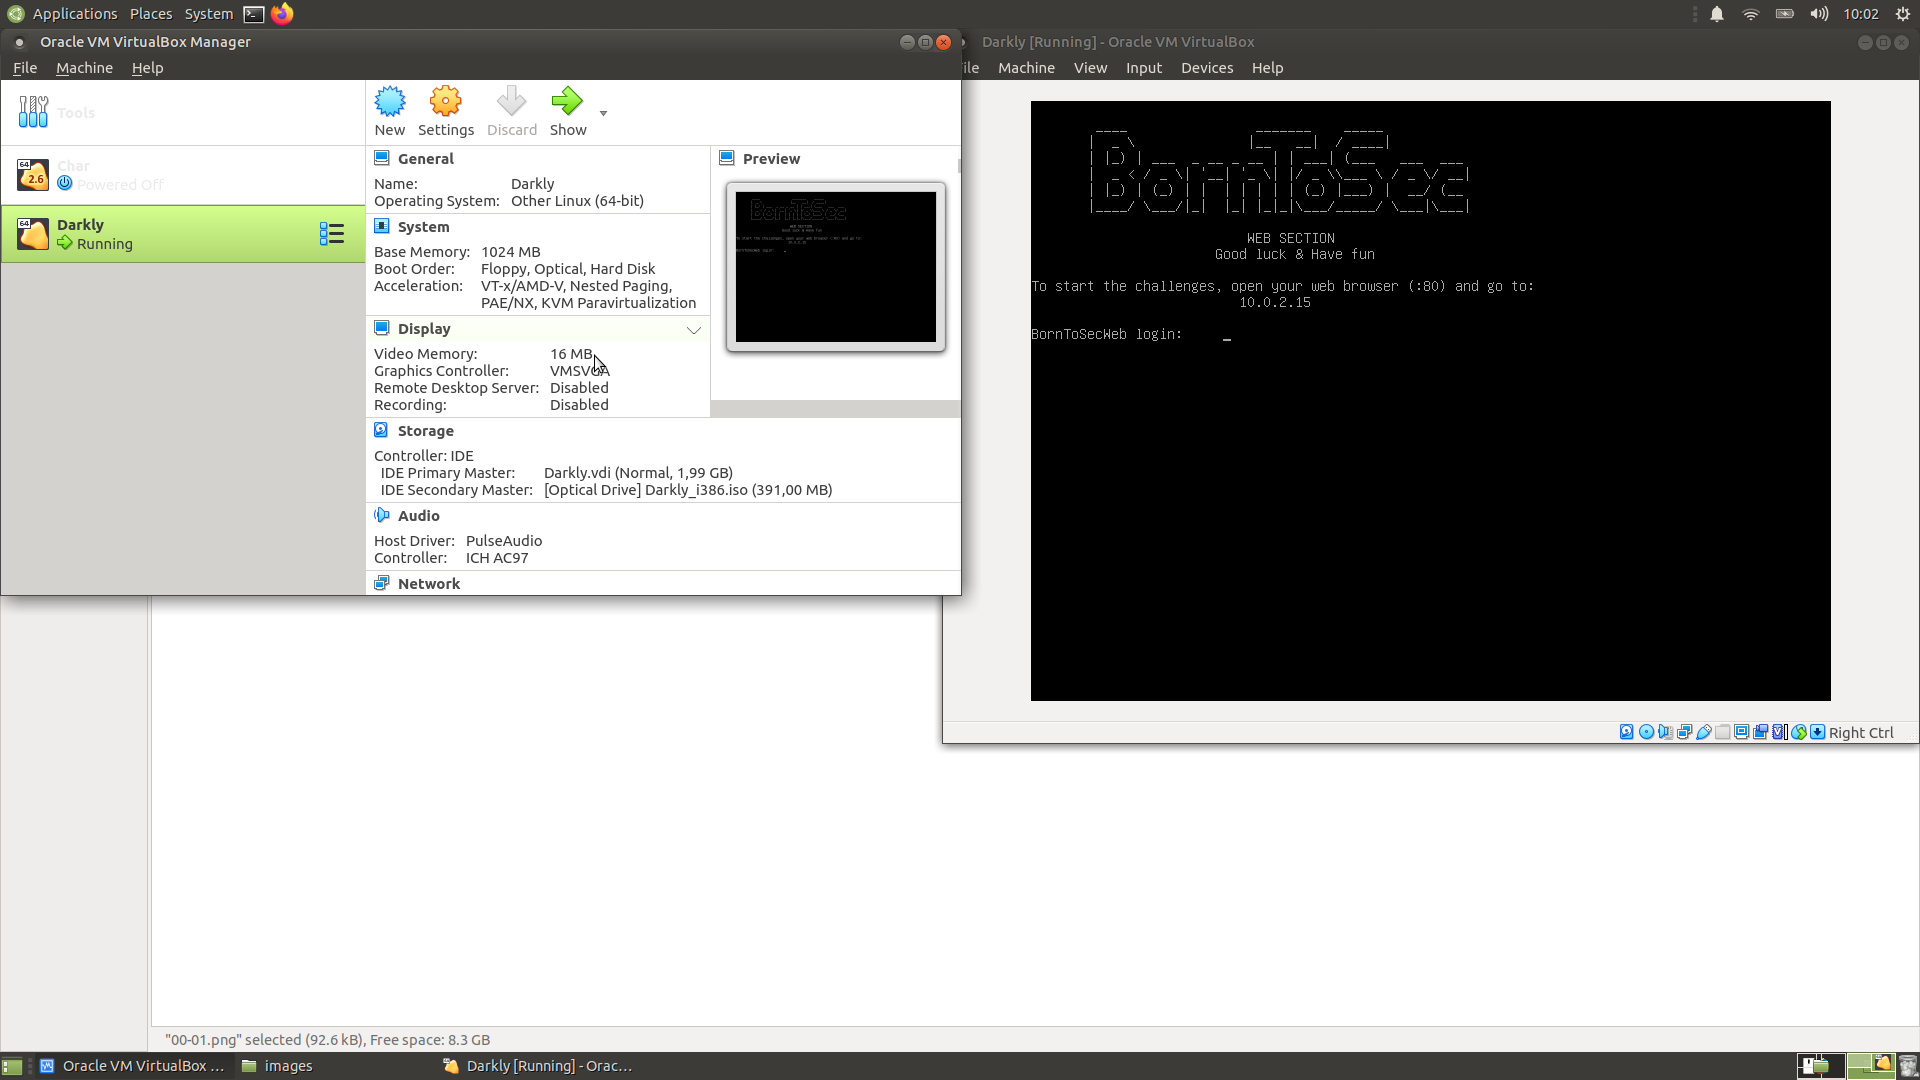
\includegraphics[width=0.752\textwidth]{images/00-09.png}\\[0cm]  
    \caption[Virtual Box]{\emph{Virtual Box Landing}, on Ubuntu}
    %from \url{http://localhost:3000/}).} % The text in the square bracket is the caption for the list of figures while the text in the curly brackets is the figure caption
    \label{fig:00-09 - Linux Virtual Box Landing} 
\end{figure}

Tell the system to use Linu
\subsubsection{Linux}

\begin{figure}[!htb]
    \centering
    %\insertcode{Scripts/example.pl}{Nena would be proud.} % The first argument is the script location/filename and the second is a caption for the listing
    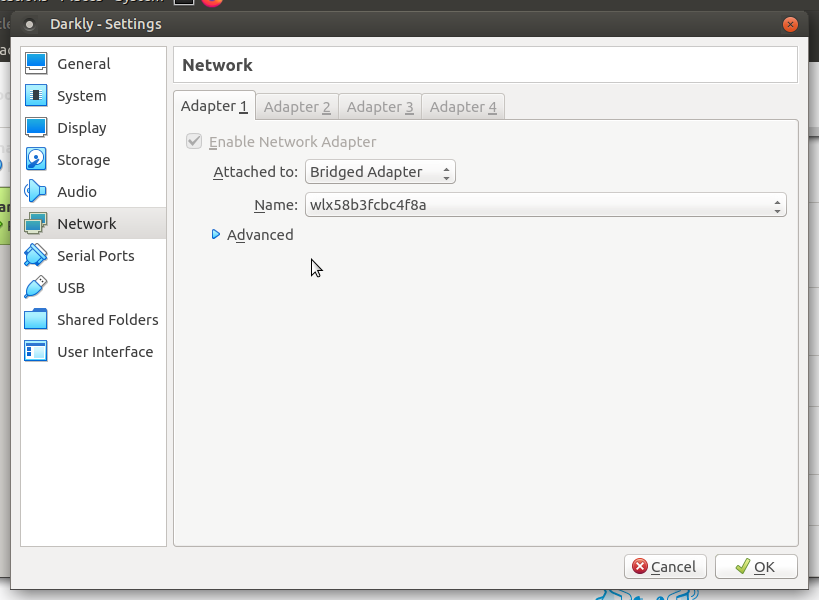
\includegraphics[width=0.752\textwidth]{images/00-10.png}\\[0cm]  
    \caption[Virtual Box]{\emph{Virtual Box Landing}, on Ubuntu}
    %from \url{http://localhost:3000/}).} % The text in the square bracket is the caption for the list of figures while the text in the curly brackets is the figure caption
    \label{fig:00-10 - Linux Virtual Box Landing} 
\end{figure}

Tell the system to use Linu
\subsubsection{Linux}

\begin{figure}[!htb]
    \centering
    %\insertcode{Scripts/example.pl}{Nena would be proud.} % The first argument is the script location/filename and the second is a caption for the listing
    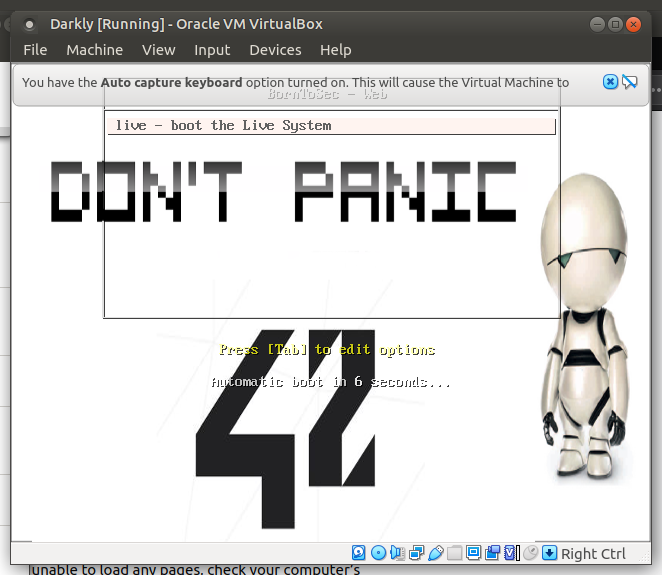
\includegraphics[width=0.752\textwidth]{images/00-11.png}\\[0cm]  
    \caption[Virtual Box]{\emph{Virtual Box Landing}, on Ubuntu}
    %from \url{http://localhost:3000/}).} % The text in the square bracket is the caption for the list of figures while the text in the curly brackets is the figure caption
    \label{fig:00-11 - Linux Virtual Box Landing} 
\end{figure}

Tell the system to use Linu

\subsubsection{Linux}

\begin{figure}[!htb]
    \centering
    %\insertcode{Scripts/example.pl}{Nena would be proud.} % The first argument is the script location/filename and the second is a caption for the listing
    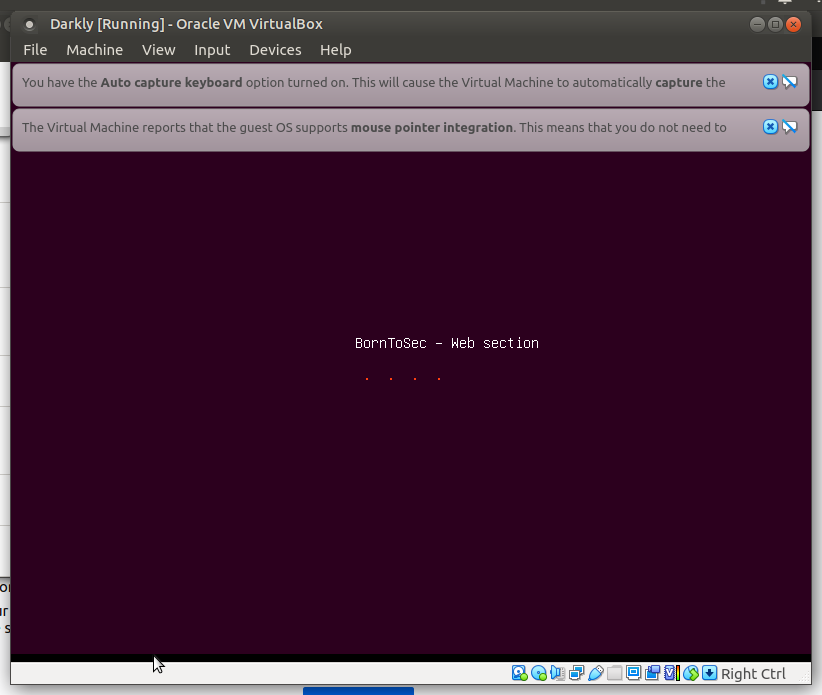
\includegraphics[width=0.752\textwidth]{images/00-12.png}\\[0cm]  
    \caption[Virtual Box]{\emph{Virtual Box Landing}, on Ubuntu}
    %from \url{http://localhost:3000/}).} % The text in the square bracket is the caption for the list of figures while the text in the curly brackets is the figure caption
    \label{fig:00-12 - Linux Virtual Box Landing} 
\end{figure}

Tell the system to use Linu
\subsubsection{Linux}

\begin{figure}[!htb]
    \centering
    %\insertcode{Scripts/example.pl}{Nena would be proud.} % The first argument is the script location/filename and the second is a caption for the listing
    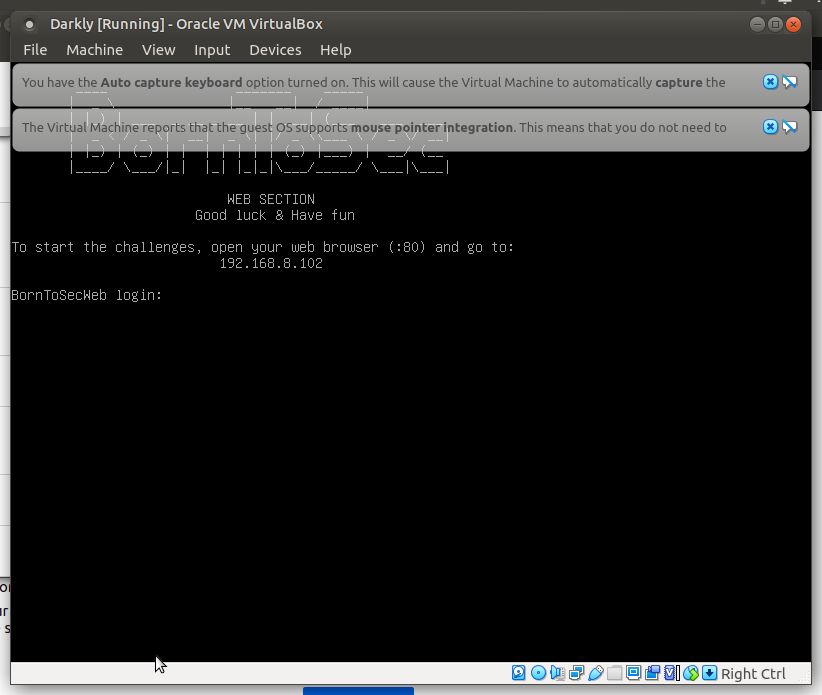
\includegraphics[width=0.752\textwidth]{images/00-13.png}\\[0cm]  
    \caption[Virtual Box]{\emph{Virtual Box Landing}, on Ubuntu}
    %from \url{http://localhost:3000/}).} % The text in the square bracket is the caption for the list of figures while the text in the curly brackets is the figure caption
    \label{fig:00-13 - Linux Virtual Box Landing} 
\end{figure}

Tell the system to use Linu
\subsubsection{Linux}

\begin{figure}[!htb]
    \centering
    %\insertcode{Scripts/example.pl}{Nena would be proud.} % The first argument is the script location/filename and the second is a caption for the listing
    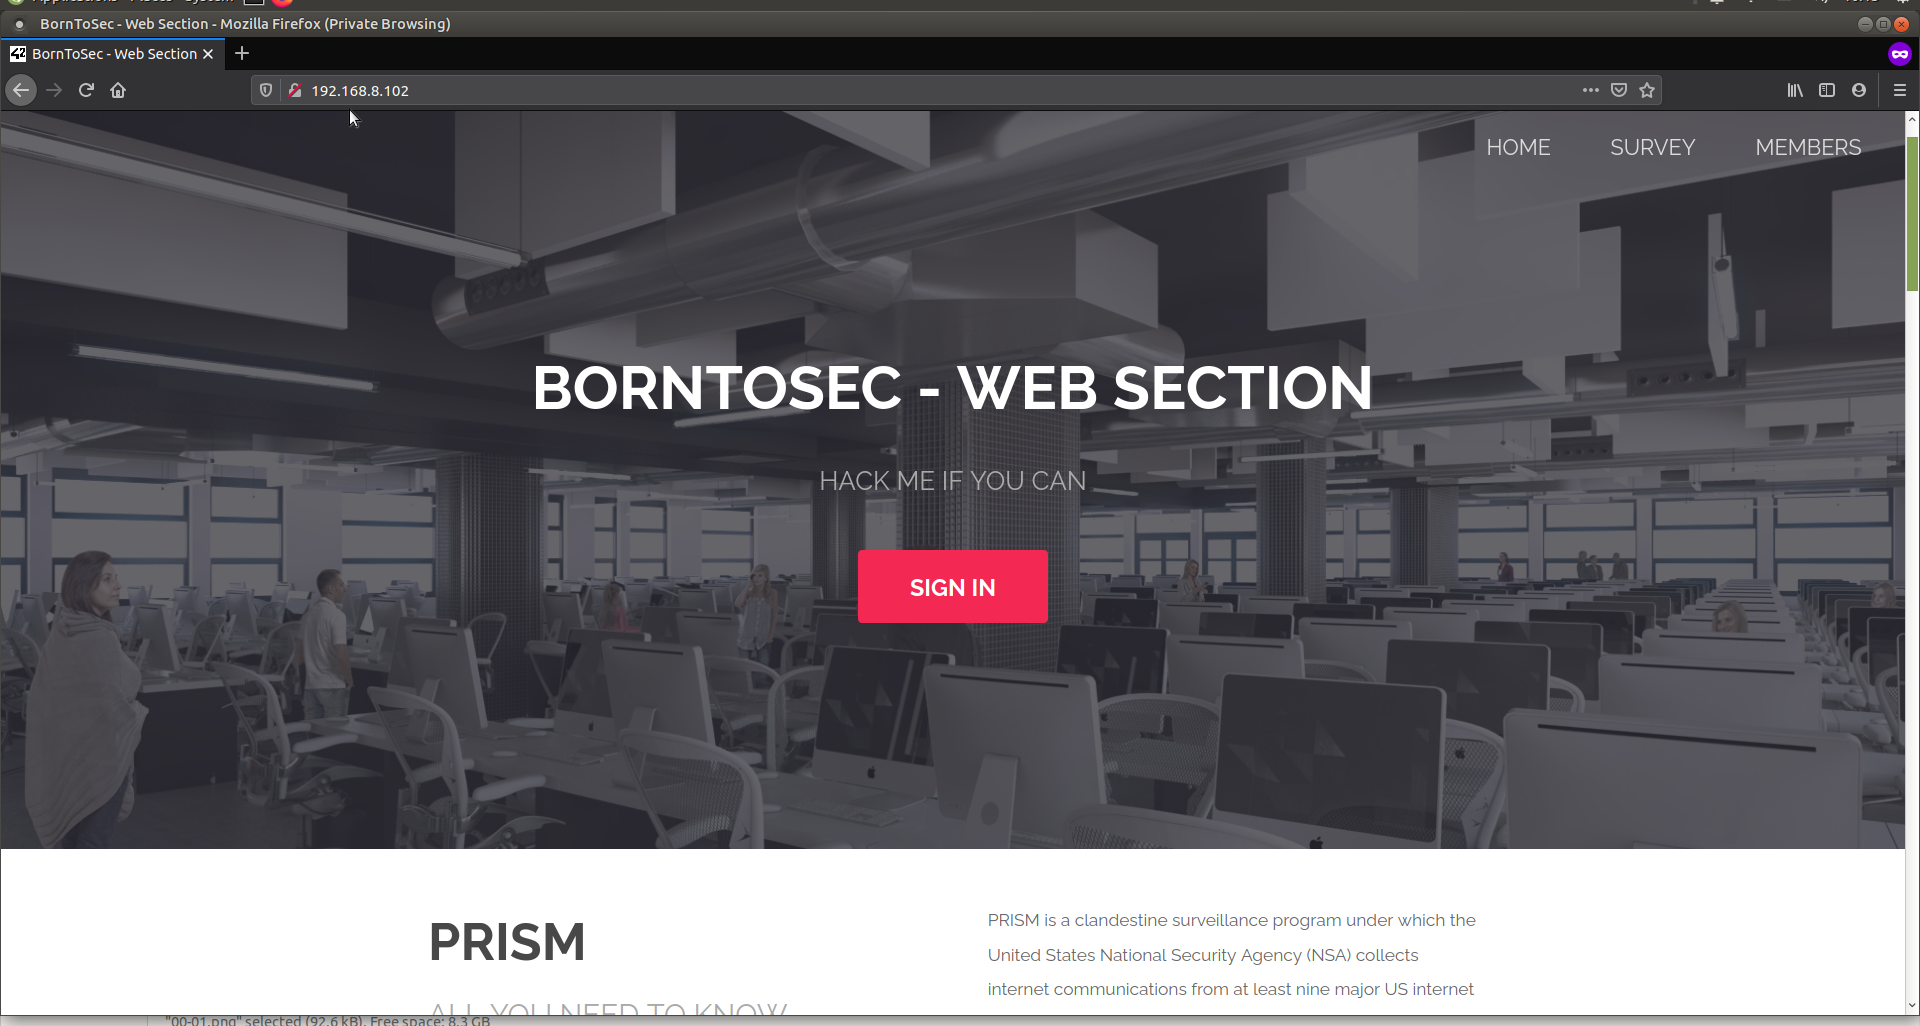
\includegraphics[width=0.752\textwidth]{images/00-14.png}\\[0cm]  
    \caption[Virtual Box]{\emph{Virtual Box Landing}, on Ubuntu}
    %from \url{http://localhost:3000/}).} % The text in the square bracket is the caption for the list of figures while the text in the curly brackets is the figure caption
    \label{fig:00-14 - Linux Virtual Box Landing} 
\end{figure}

Tell the system to use Linu
\clearpage
%\vfill
\subsection{MacOS}
At the time of typing this document a Mac was not available to conduct testing
but the documentation\cite{Docker:Mac_Install} does have instructions

%----------------------------------------------------------------------------------------

%\newpage % Start the article content on the second page, remove this if you have a longer abstract that goes onto the second page


%----------------------------------------------------------------------------------------
%	Flag \#01
%----------------------------------------------------------------------------------------

\section{Flag \#01}
%A statement requiring citation \cite{Figueredo:2009dg}.

%\newpage

%----------------------------------------------------------------------------------------
%	Flag \#02
%----------------------------------------------------------------------------------------

\section{Flag \#02}

%\input{2.method/method.tex}

A Section or subsection covering extensively unit testing will be key either here or on it's own chapter
\newpage
%----------------------------------------------------------------------------------------
%	Flag \#03
%----------------------------------------------------------------------------------------

\section{Flag \#03}

%\input{3.results/result.tex}
\newpage

%----------------------------------------------------------------------------------------
%	Flag \#04
%----------------------------------------------------------------------------------------

\section{Flag \#04}

%Reference to Figure~\vref{fig:snippet}. % The \vref command specifies the location of the reference

%\input{4.code_snip/code.tex}

\newpage

%----------------------------------------------------------------------------------------
%	BIBLIOGRAPHY
%----------------------------------------------------------------------------------------
\section{Bibliography}

\renewcommand{\refname}{\spacedlowsmallcaps{References}} % For modifying the bibliography heading

\bibliographystyle{unsrt}

\bibliography{0.Extras/sample.bib} % The file containing the bibliography
%\bibliography{sample2.bib}

%----------------------------------------------------------------------------------------

%\end{document}


\section{Student Honesty Declaration}

Engaging in any cheating or dishonesty in any form of assessment, 
assignment, test orexamination or other WeThinkCode\_ prescribed work 
is considered cheating and is grounds for disciplinary action.
Plagiarism, which is to present work (or a portion of work) as your 
own when it is not, isconsidered cheating and is not accepted at 
WeThinkCode\_.

An evaluator can flag one for plagiarism on one of the following grounds\
:\begin{itemize}
     
\item The evaluator (marker) identifies that the student does not understand
all or part of the work they have submitted.
\item If all or part of the work presented is plagiarised ,i.e. copied from 
another source without reference.
\end{itemize}

\begin{large}\textbf{Cheating in group projects}\end{large}\\

The main purpose for a group project is to give students the experience of working in ateam, by coming up with a solution to a problem together.
\begin{itemize}
    \item Each member must be able to show which portion of the project they worked on. 
    \item Failure to do so will result in the student being flagged for cheating which will begrounds for disciplinary action.
    \item This is to avoid single members doing the majority of the group project at the benefit of a member who is not contributing.
    \item In this way we are able to ensure fair assessment of each WTC\_ student’s competence.
\end{itemize}    
Group projects can be approached in two ways.
\begin{enumerate}
    \item Divide and conquer: This is usually preferred and advised when working on big projects. The project is divided into segments, in which each member of the group can accomplish. Once completed, the group will then integrate the segments to complete the project
    \item One for all: This method is usually preferred and advised when a group is working on a small project. The group will work on the solution together from the start of the project until the end. This will require the members to move at a pace in which everyone in the team can keep up with.
\end{enumerate}    
NOTE: At the end of each group project, each member should have a general and basic understanding of the project and the solution found. This will include running,testing and explaining the solutions of the project.

\section*{Declaration}

I hereby declare that the work submitted by me and/or my group members is:
\begin{itemize}
    \item Original (not plagiarised)
    \item References listed
    \item Honest \& in Good Faith
    \item Subject to WeThinkCode\_policies
\end{itemize}

\vspace{15mm}

% \begin{minipage}{0.4\textwidth}
%     \begin{flushleft}
%         \large
%         \line(1,0){120}\\
%         Mosima \textsc{Mamaleka} % Your name
%         \textit{WeThinkCode\_ Student}\\
%     \end{flushleft}
% \end{minipage}
% ~
% \begin{minipage}{0.4\textwidth}
%     \begin{flushright}
%         \large
%         \line(1,0){120}\\
%         Sibonelo \textsc{Nkosi} % Supervisor's name
%         \textit{WeThinkCode\_ Student}\\
%     \end{flushright}
% \end{minipage}

\begin{flushleft}
\line(1,0){120}\\
Sibonelo \textsc{Nkosi}\\ % Your name
Username: \textsc{sinkosi}\\ % Your name
{\large\textit{Developer}}
\end{flushleft}


%---------------------------------------------------------------------------------------
%\printindex

\end{document}